\documentclass[journal = jacsat, manuscript=article, layout = twocolumn]{achemso}

\listfiles
\author{Benjamin Ab\'ecassis} 
\email{benjamin.abecassis@u-psud.fr}
\affiliation{Laboratoire de Physique des Solides, Univ. Paris-Sud, CNRS, UMR 8502, F-91405 Orsay Cedex, France}

\author{C\'ecile Bouet}
\affiliation{Laboratoire de Physique et d'Etude des Mat\'eriaux, CNRS, Université Pierre et Marie Curie, ESPCI, 10 rue Vauquelin, 75005, Paris,}


\author{Mickael D. Tessier}
\affiliation{Laboratoire de Physique et d'Etude des Mat\'eriaux, CNRS, Université Pierre et Marie Curie, ESPCI, 10 rue Vauquelin, 75005, Paris,}

\author{Patrick Davidson}
\affiliation{Laboratoire de Physique des Solides, Univ. Paris-Sud, CNRS, UMR 8502, F-91405 Orsay Cedex, France}

\author{Benoit Dubertret}
\affiliation{Laboratoire de Physique et d'Etude des Mat\'eriaux, CNRS, Université Pierre et Marie Curie, ESPCI, 10 rue Vauquelin, 75005, Paris,}



%\title{On the stacking and colloidal stability CdSe nanoplatelets}%
%\title{Lamellar order in stacks of CdSe nanoplatelets}
\title{Solution self-assembly of CdSe nanoplatelets into stacks with a lamellar order}
\title{Structure of CdSe Nanoplatelets and their stacking in solution : a SAXS study}


\begin{document}

\begin{abstract}
\end{abstract}

\section{Introduction}

Self assembly of anisotropic nanoparticles \cite{Glotzer:2007ib}. Among them nanoplatelets are particularly interesting \cite{Saunders:2006hu,Paik:2011if,Ye:2013dh,Jones:2011ba,Young:2012wv}.

Semi-conducting colloidal nanoplatelets have been discovered recently \cite{Ithurria:2011jt,*Ithurria:2011bi,*Ithurria:2008fz} and are arousing interest for their original optical properties \cite{Tessier:2012js} and their potential applications in optoelectronics or photovoltaics applications. In spherical quantum dots, the quantum confinement which leads to the reduction of the band gap energy occurs in the three spatial dimensions. Hence, the electron-hole pair is confined in all the directions. In the case of nanoplatelets, the confinement is limited to one direction in space since the dimension of the platelets lies below the Bohr radius in one dimension only. Since, the thickness of the platelets can be controlled at the atomic level, the degree of confinement and hence the band gap can be finely tuned. 

These nanoparticles are synthesized in solution, through the reaction of cadmium and selenium precursors in the presence of ligands (long chain carboxylic acids) which adsorb on the cadmium rich (001) surface of the nanoparticle and make them dispersible in apolar solvants such as hexane or toluene. While it has been observed that cadmium acetate is a necessary component for the two dimensionnal growth to occur, the relative concentration in platelets of  the different thicknesses and their lateral extension depends on other parameters of the synthesis such as the reaction temperature, the concentration in precursors and ligands or the injection speed of the metal precursors. Three populations of nanoplatelets have been synthesized to date which emit at 463, 513 and 550 nm. These correspond to thicknesses of 0.9, 1.5 and 2.1 nm. More importantly, colloidal solution containing only one population of platelets can be prepared. 

Here we study the self assembly of 510 nanoplatelets in solution. Using TEM we can only probe one or several monolayers of nanoparticle and not study self assembly in bulk. On the contrary SAXS is an ideal technique to probe self assembly in solution. It enables the determination of the strucutre over macroscopic (micrometers) area for length scales from 1 to 100 nm.  





\section{Experimental section}
\textbf{\textit{Chemicals}} : Cadmium acetate dihydrate (Cd(OAc)$_2$.2H$_2$O), technical grade 1-octadecene (ODE), myristic acid sodium salt, oleic acid (OA) and selenium in powder were purchased from Sigma-Aldrich. Ethanol and hexane were purchased from SDS Carlo-Erba.\\

\textbf{\textit{Nanoplatelets synthesis}} : The cadmium myristate salt was synthesized as described in details elsewhere \cite{Yang:2005kc}. For the nanoplatelet synthesis : 0.234 g of cadmium myristate and 0.024 g of selenium powder were mixed with 30 mL of octadecene in a three-neck round-bottom flask equipped with a condenser, a septum and a temperature controller . Under magnetic agitation, the mixture was then degassed under vacuum for 30 minutes and heated from ambient temperature to 240$^\circ$C. When the temperature reached 200$^\circ$C (after about 6 min 30 s) 0.160 g of cadmium acetate (in powder) was added to the solution after having withdrawn the septum. When the salt is poured in the solution, the solution's color is yellow and starts to turn red. After 12 min at 240$^\circ$C, heating was stopped and 1 mL of oleic acid is added. At this stage, the solution contained, as shown by UV-vis absorption, three populations of nanoparticles : platelets emitting at 460 nm, platelets emitting at 510 nm and quantum dots. To isolatethe platelets emitting at 510 nm, a series of selective precipitation/centrifugation was performed. The raw product was sperated in two centifuge tube and 20 mL of ethanol was added to each of the tubes. After centrifuation for 10 min at 5000 tr/min. The supernatant contained quantum dots while the precipitate only platelets. The latter was re-dispersed in hexane and this solution was centrifuged at 3000 tr/min for 10 minutes . The supernatant only contained platelets emitting at 510 nm while the larger platelets emitting at 460 nm precipitated. At last, ethanol was added to the solution to make the platelet precipitate, the supernatant was discarded and the precipitate was redispersed in hexane.\\

\textbf{\textit{Small Angle X-ray Scattering}} : SAXS experiments were performed at the SWING beamline of the SOLEIL synchrotron (Saint-Aubin, France). Measurements were carried out using a fixed energy of 12 keV and three sample to detector positions (0.85, 1.07 and 6.56 m). The typical accessible range of scattering vector modulus q was 0.02 – 10 nm$^{−1}$ ($q=\frac{4\pi}{\lambda} \sin(\theta)$), where 2θ is the scattering angle and $\lambda$ = 1.033 \AA  the wavelength). Scattering patterns were recorded on an AVIEX 170170 CCD camera formed by four detectors and radially averaged.\\

\textbf{\textit{Transmission Electron Microscopy}} : TEM samples were prepared by deposing a drop of the nanoparticle dispersion on a carbon coated copper grid and let dry in air. 																					

\section{Results and discussion}
\begin{figure}	
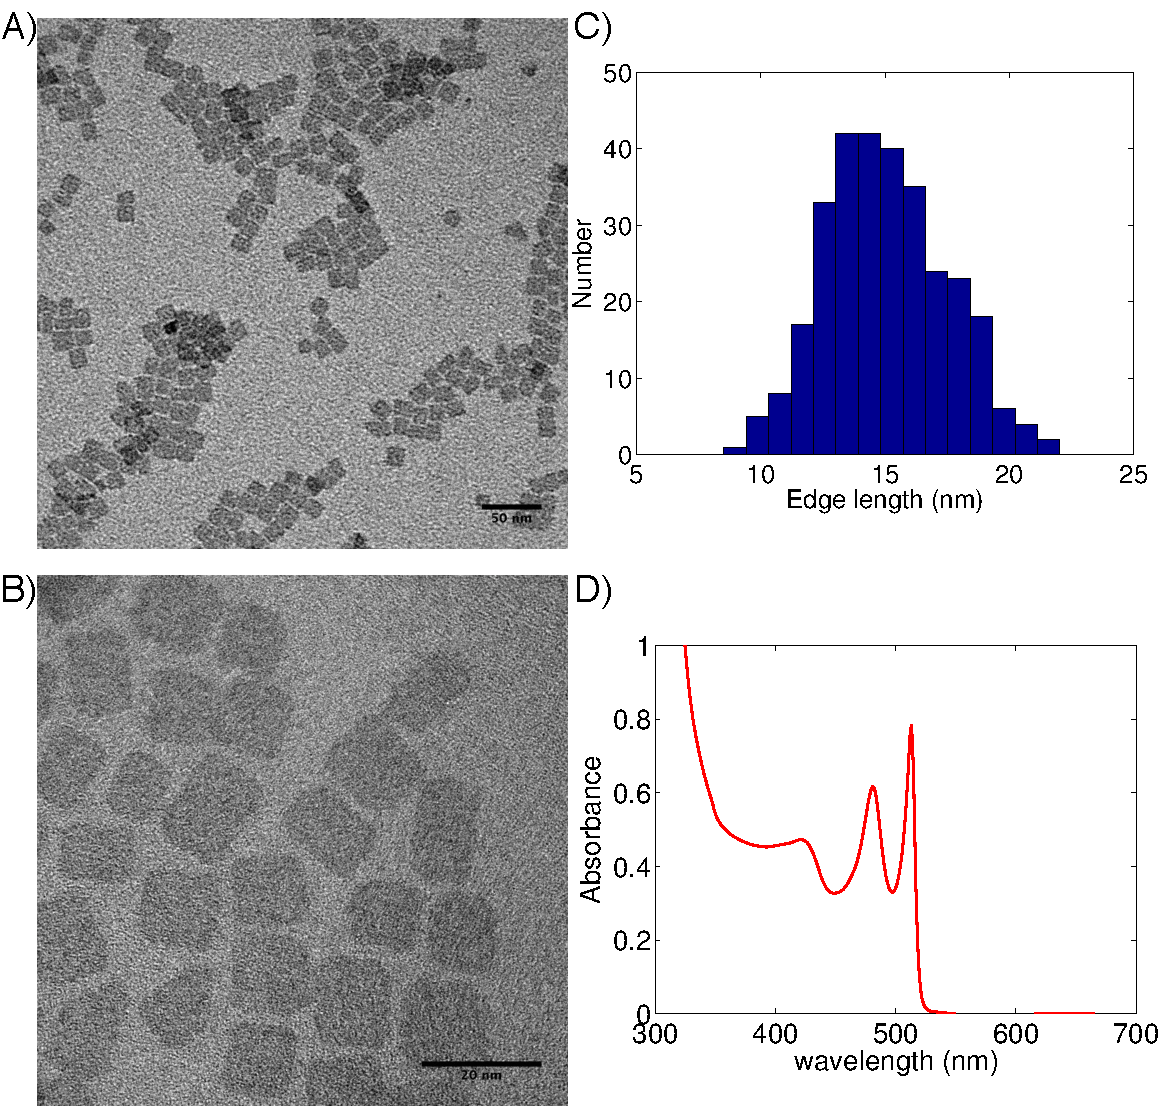
\includegraphics[width = \linewidth]{/Users/abecarix/Boulot/CdSe/article_benjamin/figures/figure1/figure1.pdf}
\caption{\label{TEM_UV} A) and B) represent TEM micrograph of the CdSe nanplatelets as synthesized. Scale bars are 50 nm for A) and 20 nm for B). C) Histogram of the edge length measured on 150 nanoparticles. D) Absorption (red) and emission spectra (blue) avec the diluted platelet dispersion.}
\end{figure}

\subsection{Description of the nanoplatelets alone}
TEM images of the as-synthesized CdSe nanoplatelets dispersed in hexane are showns on figure \ref{TEM_UV}. The low magnification micrographs show that the nanoplatelets are homogeneously dispersed on the substrate and that they stand with their small dimension (their thickness is around 1.5 nm) perpendicular to the substrate. At higher magnification, we observe that the platelets have a rectangular shape with sharp edges and long edges with dimensions comprised between 10 and 20 nm. Measuring 150 nanoparticles by hand yields an average edge length of 15.0 nm with an standard deviation of 2.5 nm (figure \ref{TEM_UV}.C). The UV-VIS absorption and the emission spectra (figure \ref{TEM_UV}.D) are characteristic of CdSe nanoplatelets \cite{Ithurria:2011jt} with sharp peaks in the absorption spectrum  and a single strong emission line at 513 nm. Since we do not observe emitted intensity beyond the 513 nm line, we can deduce that no quantum dots or other population of nanoplatelets are present in the sample. Since the nanoparticles are all oriented with their small dimension perpendicular to the TEM grid, it is difficult to estimate their thickness from these TEM experiments. To achieve a quantitative measurement of the thickness of the nanoplatelets in solution we conducted high resolution SAXS experiment. \\

A radially averaged SAXS pattern of a colloidal solution of the nanoplatelets dispersed in hexane is shown on figure \ref{SAXS_plaq}. At low scattering vector $\bf{q}$ the monotonous decrease of the scattered intensity indicate that there is no visible interaction between the platelets in solution. The modulation of the intensity at higher $q$ corresponds to distances in real space comprised between and 1.4 nm and 0.8 nm. Hence, we hypothesize that this oscillation is due to the thickness of the nanoplatelets. In order to get a more quantitative estimate, we fitted the experimental intensity to a model of disks with a small polydispersity in thickness (see Methods section). Three different populations were considered with average thicknesses of 1.22, 1.52 and 1.82 nm. These values correspond to respectively 4,5 and 5 half unit-cells of the zinc-blind CdSe with a 0.608 nm lattice parameter. From figure \ref{SAXS_plaq}, it is clear that the theoretical case which is closer to the experimental data corresponds to platelets with an average thickness of 1.52 nm. In the two other cases, the theoretical scattered intensity decrease either at too small or at two high scattering vectors and do not reproduce the experimental bump. This result also confirm that the nanoplatelet population is monodiperse since the theoretical modeling yields a full width at half maximum of 0.135 nm (less than 10\% of the average thickness). 


\begin{figure}
\begin{center}
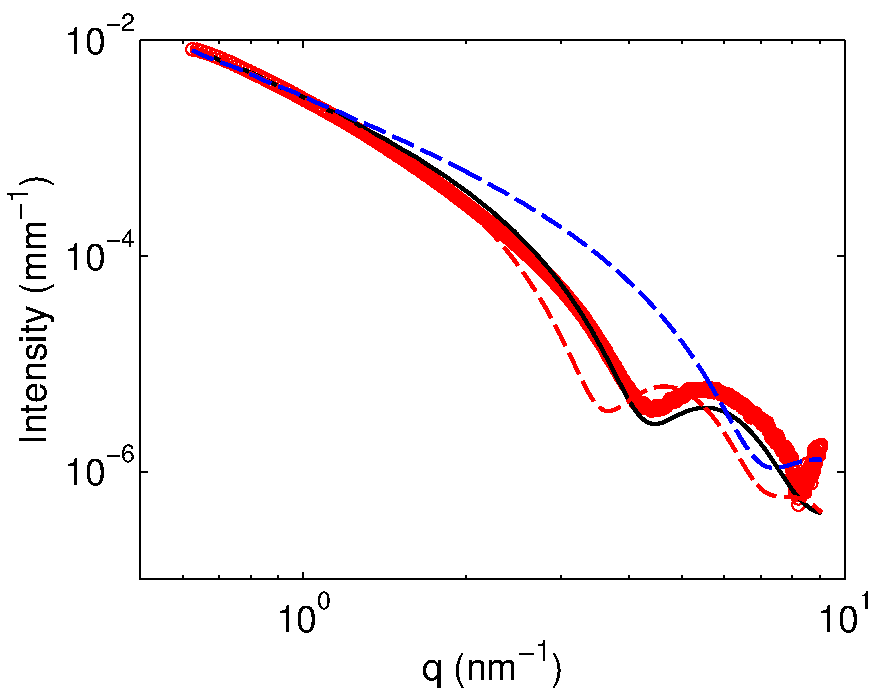
\includegraphics[width=\linewidth]{/Users/abecarix/Boulot/CdSe/article_benjamin/figures/fit.pdf}
\caption{\label{SAXS_plaq}}
\end{center}
\end{figure}


\subsection{Stacks of nanoplatelets}
When a colloidal platelet solution is kept in a glovebox, its translucid aspect is preserved and we do not observe any trace of precipitate or turbidity over months. Hence, away from air moisture the platelets are well dispersed in solution and do not aggregate. On the contrary, when the vial is subjected to multiple open and closing or when a small amount of anti-solvent such as ethanol is added to the hexane solution, the colloidal solution is not stable anymore and a precipitate appears at the bottom of the vial. The kinetics of the destabilisation of the colloid depends on the precise experimental conditions and ranges from seconds when a significant proportion of the anti-solvant is added to weeks when the vial is just kept in air without further protection. In order to better understand the structure of the precipitate, they were transferred in glass capillaries and probed using SAXS. Figure \ref{stacks} presents SAXS patterns for the a stable NPLs solution and for their self-assembled precipitate. Surprisingly, we note that intense Bragg peaks are visible in the radially averaged intensity. These peaks correpond to rings in the 2D scattering pattern visible in the inset. Two populations of peaks are observed. The structure factor (S(q), see inset of figure \ref{stacks}) is obtained as $I_s(q)/I_p(q)$ where $I_s(q)$ and $I_p(q)$ are the background corrected scattering patterns of the stacked platelets and the free particles respectively. The position and full width at half maximum of the peaks are determined through lorentzian fitting of the structure factor. A Scherrer analysis of the peaks yiels a domain size of XX nm \cite{Smilgies:2009et}


\begin{figure}
\begin{center}
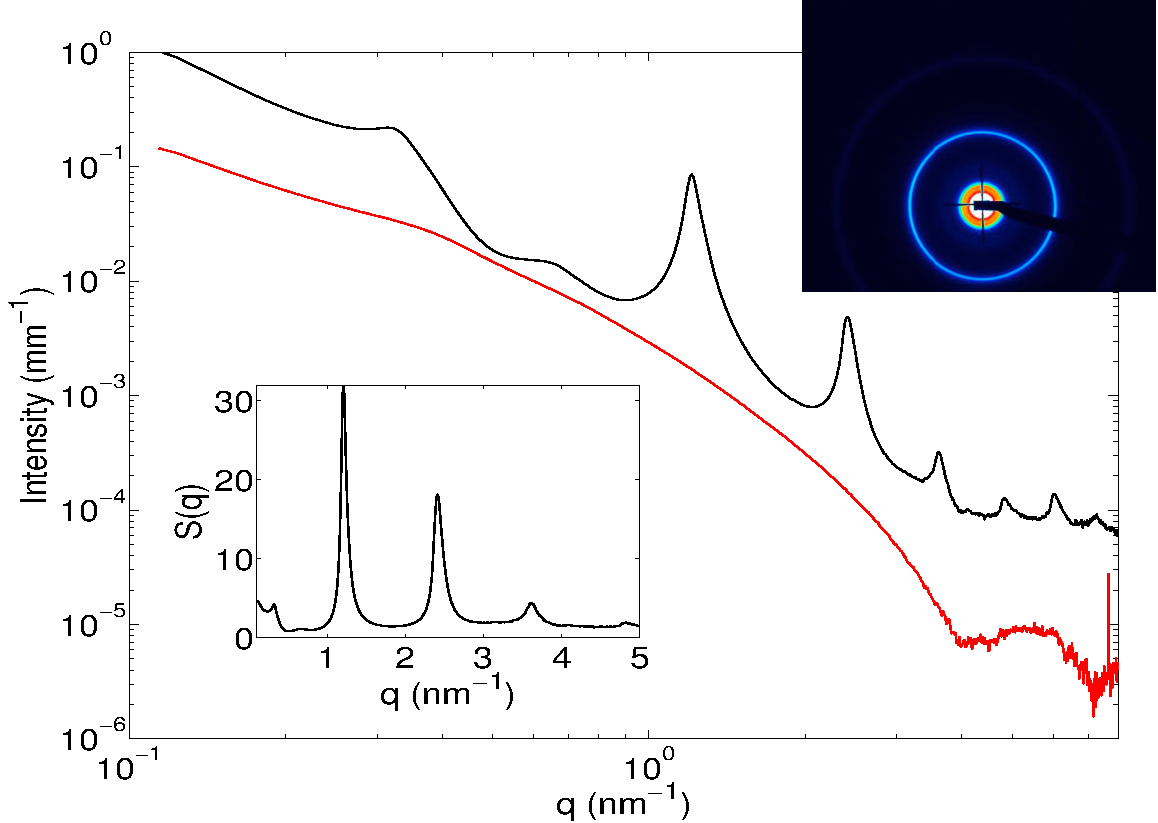
\includegraphics[width=\linewidth]{/Users/abecarix/Boulot/CdSe/article_benjamin/figures/sqwim.pdf}
\caption{\label{stacks} SAXS patterns of stacked (black cuvre) and unstacked (red curve) CdSe nanoplatelets. Top inset : 2D SAXS image of the stacked nanoplatelets. Note the presence of rings in the pattern. Bottom inset : structure factor the stacked platelets}
\end{center}
\end{figure}

A liquid structure factor is much too shallow to represent the experimental data. In a real long range order the FWHM would be constant over the order of the Bragg reflexion whereas it decrease in the present case \cite{guinier_book}. Hence we are in an intermediate state between a liquid and a solid with a long range order (definition of a liquid crytal ??).

Effect of the addition of ethanol on the colloidal stability. When we add ethanol to the solution we see that, at a given quantity, the solution becomes turbid. This is due to the apparation of large micronic flocculates. To see the effect of the quantity of ethanol on the stacking we add small amounts of ethanol in a dilute solution of platelets and acquired SAXS patterns. The result are presented on figure %\ref{quantity_etoh}


We can vary the length of the ligand's alkane chain and see the effect on the interparticle distance. Discussion on the liquid character of the ligands chain which is necessary to get longer range self assembly \cite{Geyer:2012he}


\begin{figure}
\begin{center}
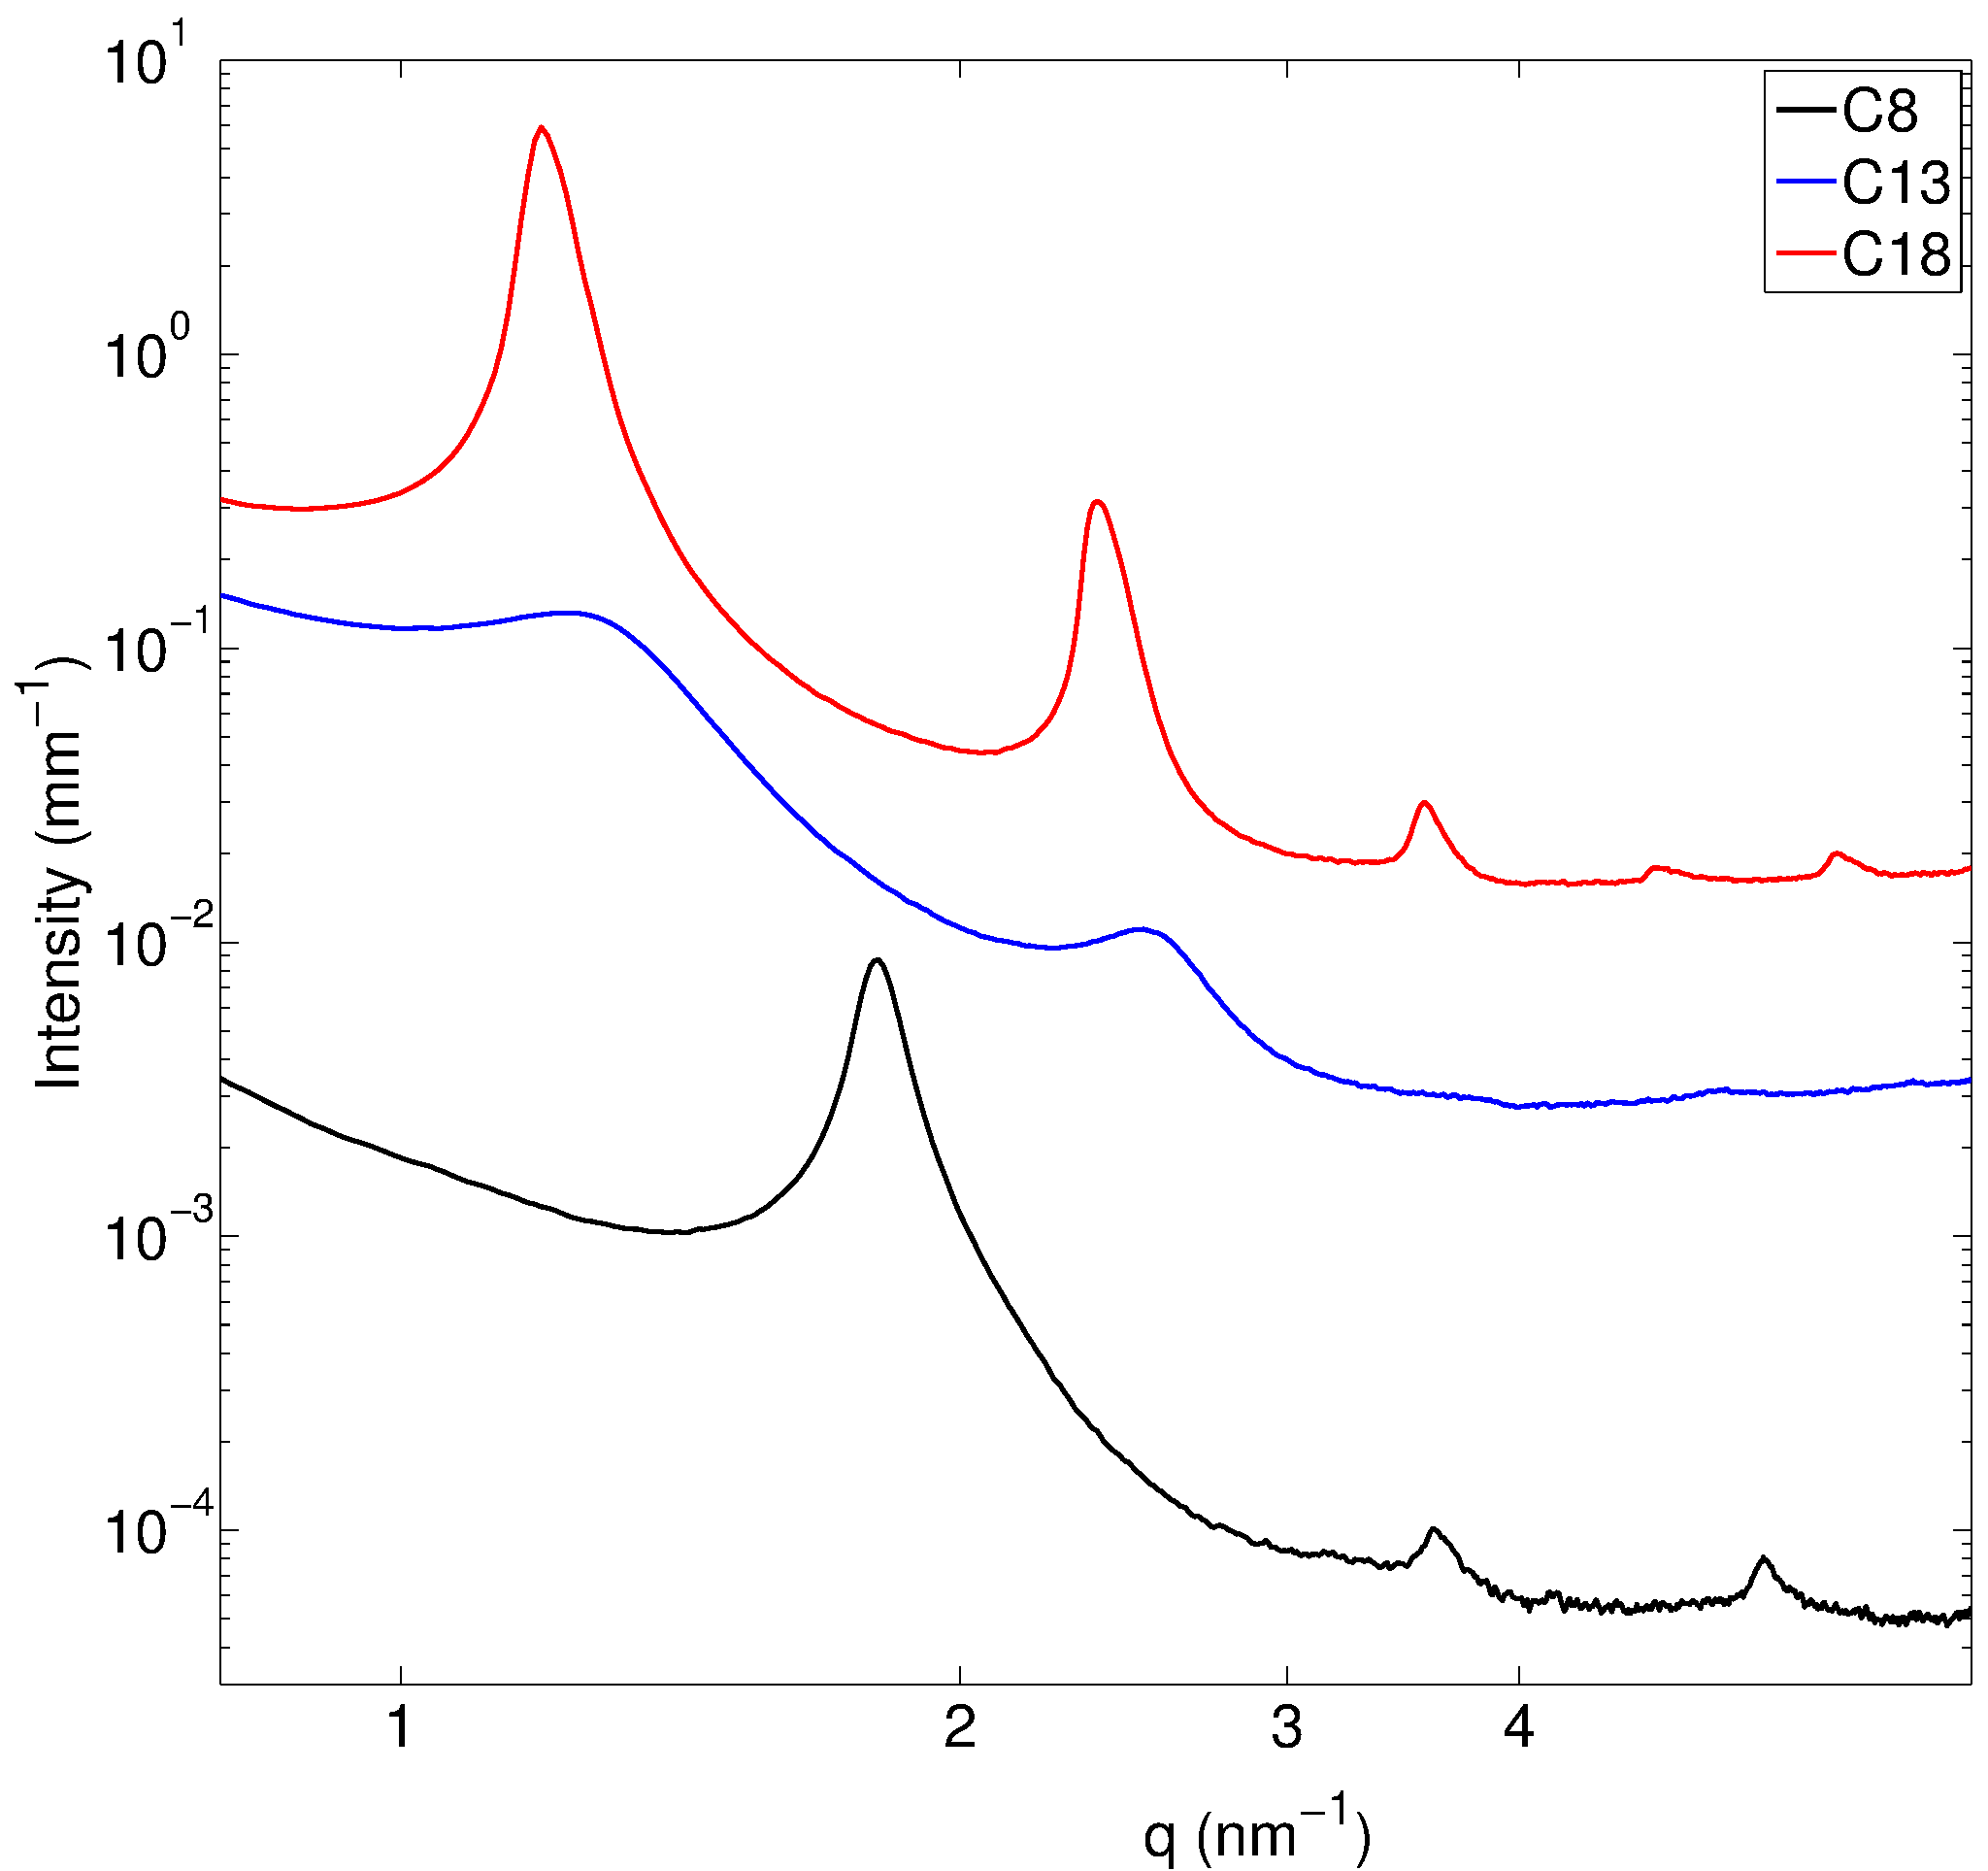
\includegraphics[width=\linewidth]{/Users/abecarix/Boulot/CdSe/article_benjamin/figures/cvar.pdf}
\caption{SAXS patterns of stacked CdSe nanoplatelets with varying ligand's chain length}
\end{center}
\end{figure}
Need a dicussion on the stripping off of the ligands. See the NMR article of Zeger Hens in ACS Nano and chem Mater.\\

Need a photograph of flocculated and dispersed nanoplatelets in solution.

Discuss the effect of water on the colloidal stability and cite golan

Discuss the effect of the chain length on

\bibliography{biblio}

\end{document}


